\section{Van der Pol Example}
\label{Van der Pol Example}


Applying the UKF to the Van der Pol oscillator will be used as a simple example to demonstrate the impacts of measurement and process noise. The Van der Pol equation, so named after its developer Balthasar van der Pol, describes a self sustaining oscillator that create energy at small amplitudes and remove energy from large amplitudes. The Van der Pol equation describes a nonconservative oscillator (also known as a relaxation oscillator). Applications of the Van der Pol oscillators include circuits, vacuums, and modeling certain biological systems. 
 \cite{weisstein_2019}. The Van der Pol oscillator is represented by a nonlinear second order differential equation: \\
\begin{align*}
\frac{d^2y}{dt^2} + \mu(y^2-1)\frac{dy}{dt} = 0
\end{align*}   \\
Here, $\mu$ is a damping coefficient. Therefore, for all $\mu < 0$, dampening occurs and the system tends to 0. The rate at which the system converges to zero is dependent on the size of $\mu$, with larger values taking longer to converge and smaller values converging much faster. If $\mu = 0$, the system becomes a simple harmonic oscillator, where motion is periodic. Lastly, if $\mu > 0$, the system enters a limit cycle.     \cite{kinoshita_2013}. \\ 

\noindent The UKF can be applied to this nonlinear system to determine where the system will be at a point in time. To do so, relevant state variables include position and velocity. Using the equation above, we are able to isolate the differential equations of these two state variables. In this case, we are assuming $\mu = 1$:\\ 

\noindent From basic differential equations, we know that: 
\begin{align*}
   y = \text{position }
  \end{align*}
 \begin{align*}
  \frac{dy}{dt}  = v = \text{velocity}
  \end{align*}
  \begin{align*}
  \frac{d^2y}{dt^2}  =  \frac{dv}{dt}  = -\mu (y^2 - 1)v - y =\text{acceleration}
  \end{align*}
  \begin{align*}
 	\frac{dv}{dt}  +\mu(y ^2-1)v + y  = \text{rewritten Van der Pol equation}
 \end{align*}
 
\newpage

\noindent State variable: let 1 and 2 be the placeholders of position and velocity
\begin{align*}
x_k = \begin{bmatrix}
          y\\ 
          v
           \end{bmatrix}  =
           \begin{bmatrix}
           1 \\
           2
           \end{bmatrix}
\end{align*}
We can use knowledge of differential equations associated with the state variables to generate the nonlinear transformation function $f$. 
\begin{align*}
f = \dot x_k  = \begin{bmatrix}
          \dot y \\
           \dot v
           \end{bmatrix}  =
           \begin{bmatrix}
           v \\
           -\mu (y^2 - 1)v - y 
           \end{bmatrix}=
           \begin{bmatrix}
           v \\
           a
           \end{bmatrix} =
           \begin{bmatrix}
           x(2) \\
          ( 1-x(2^2))x(2) - x(1)
           \end{bmatrix}
\end{align*}


\noindent In this particular example, the only measurement received from the system is position. Therefore, this filter is continually correcting for the position state state variable through measurement function $h$. Here, measurements of the system are simulated by adding noise to the position state variable. Even though there are only measurements for one state variable, we can still generate estimates of both state variables. In terms of parameters $\alpha, \kappa$, and $\beta$, default values were used.\\ 

\noindent To simulate a Van der Pol Oscillator, an ordinary differential equation solver can be applied to state function $f$ to generate true values of the system. Of course, systems do not perform perfectly; variations in model performance can be captured by randomly adding noise to the system. \\

\noindent All of this can be modeled on Matlab; all source code is complimentary of Matlab and can be referenced in Appendix A \cite{matlab /& simulink}

\begin{figure}[h]
    \centering
    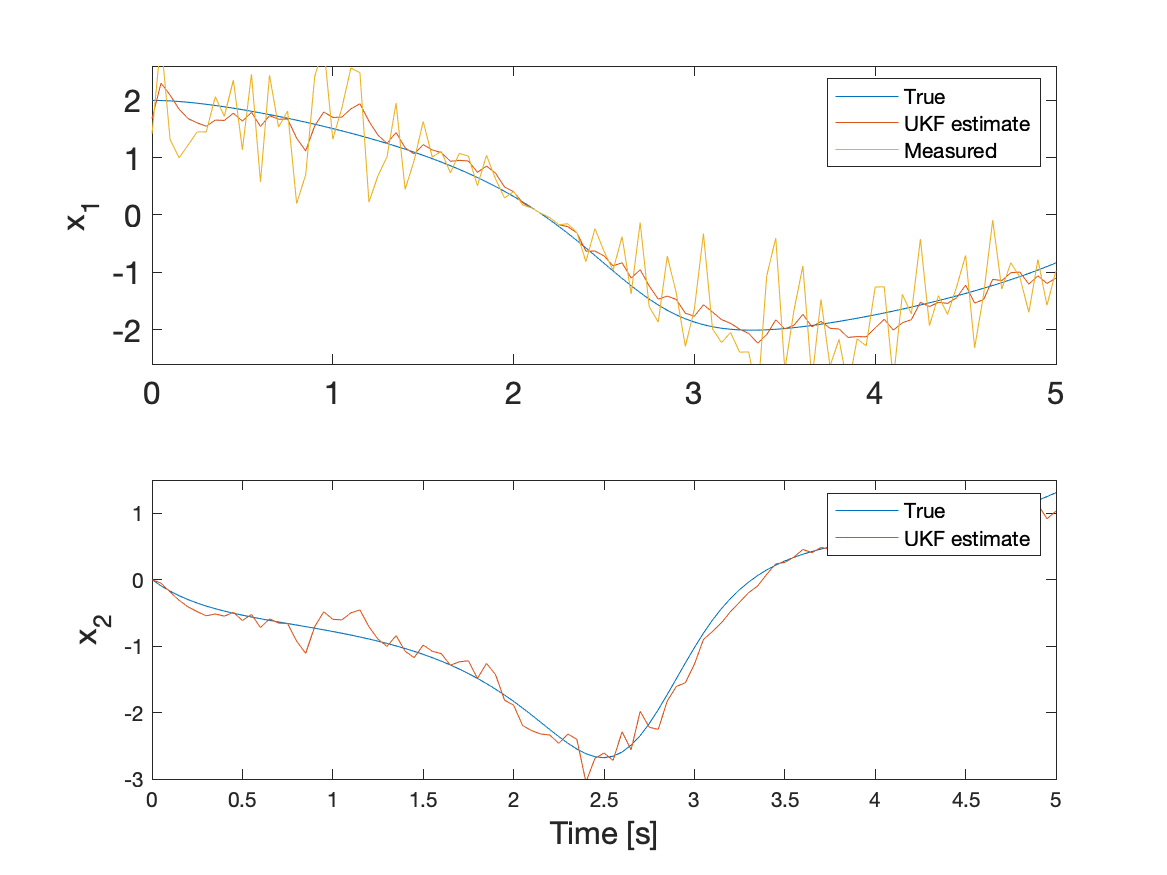
\includegraphics[scale = 0.6]{VDP.png}
    \caption{Performance of the UKF with R = 0.2, and Q = (0.02 0.1).
    As expected, the model converges on the true values of the system for both state variables. In this case, the only measurements we are receiving from the system are position, which is why the second state variable has no measured values.}
\end{figure}
\begin{figure}[h]
    \centering
    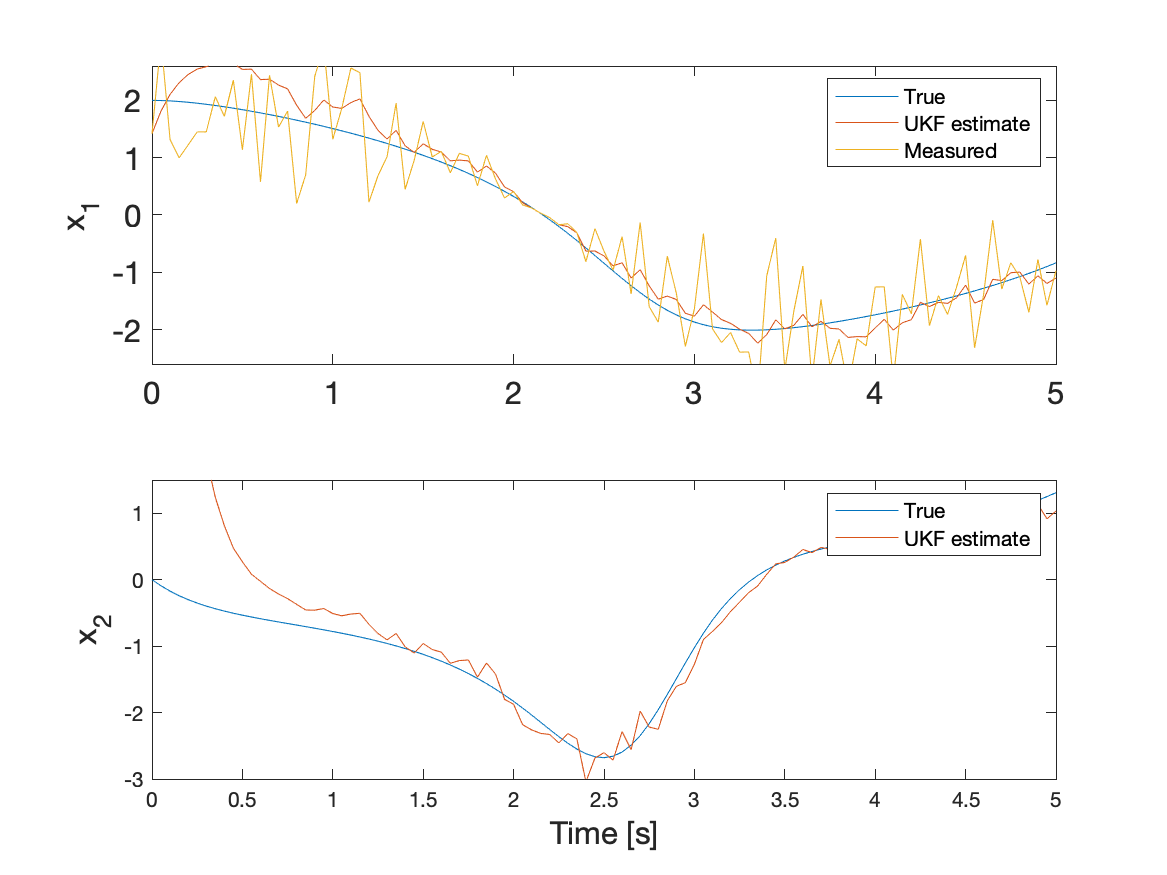
\includegraphics[scale = 0.6]{VDP_badinitial.png}
    \caption{Performance of the UKF with poor initial conditions: (1, 7)  instead of (2,0). Recall that inaccurate intial conditions cause convergence to take place more slowly. This seems to be the case, especially in the state variable that is not being corrected for.}
\end{figure}


\begin{figure}[!tbp]
  \centering
  \subfloat[UKF with high measurement noise (0.9)]{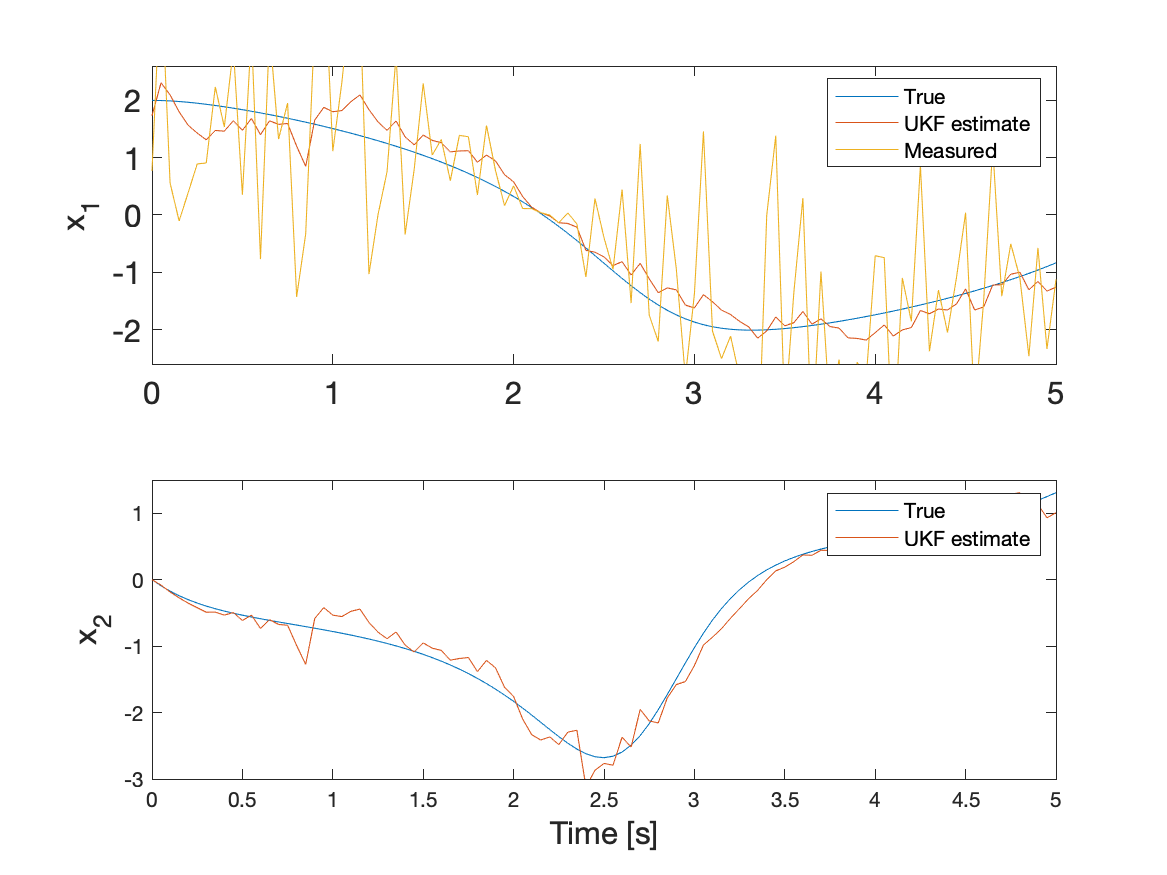
\includegraphics[width=0.5\textwidth]{VDP_highMN.png}\label{fig:f1}}
  \hfill
  \subfloat[UKF with low measurement noise (0.002)]{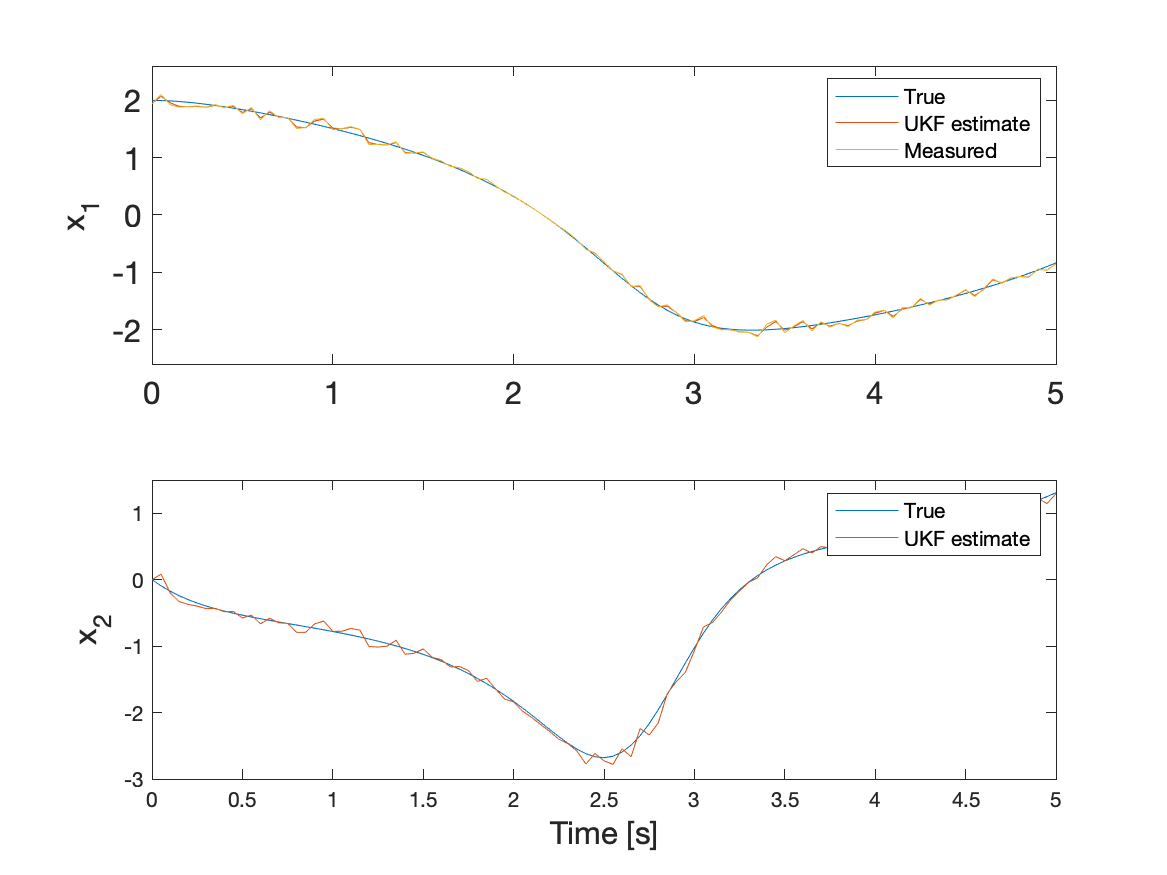
\includegraphics[width=0.5\textwidth]{VDP_lowMN.png}\label{fig:f2}}
  \caption{UKF on VDP oscillator with difference values of measurement noise.
  The model's behavior changes in response to the different values of measurement noise. Even when measurement noise is high, the UKF continues to perform well. Though, the rate of convergence appears to be slower.
On the other hand, when measurement noise is low, the UKF seems to converge instantly with the measured values. The velocity state variable also  quickly converges with the true value of the system.}
\end{figure}

\begin{figure}[!tbp]
  \centering
  \subfloat[UKF with high process noise (0.9 0.8)]{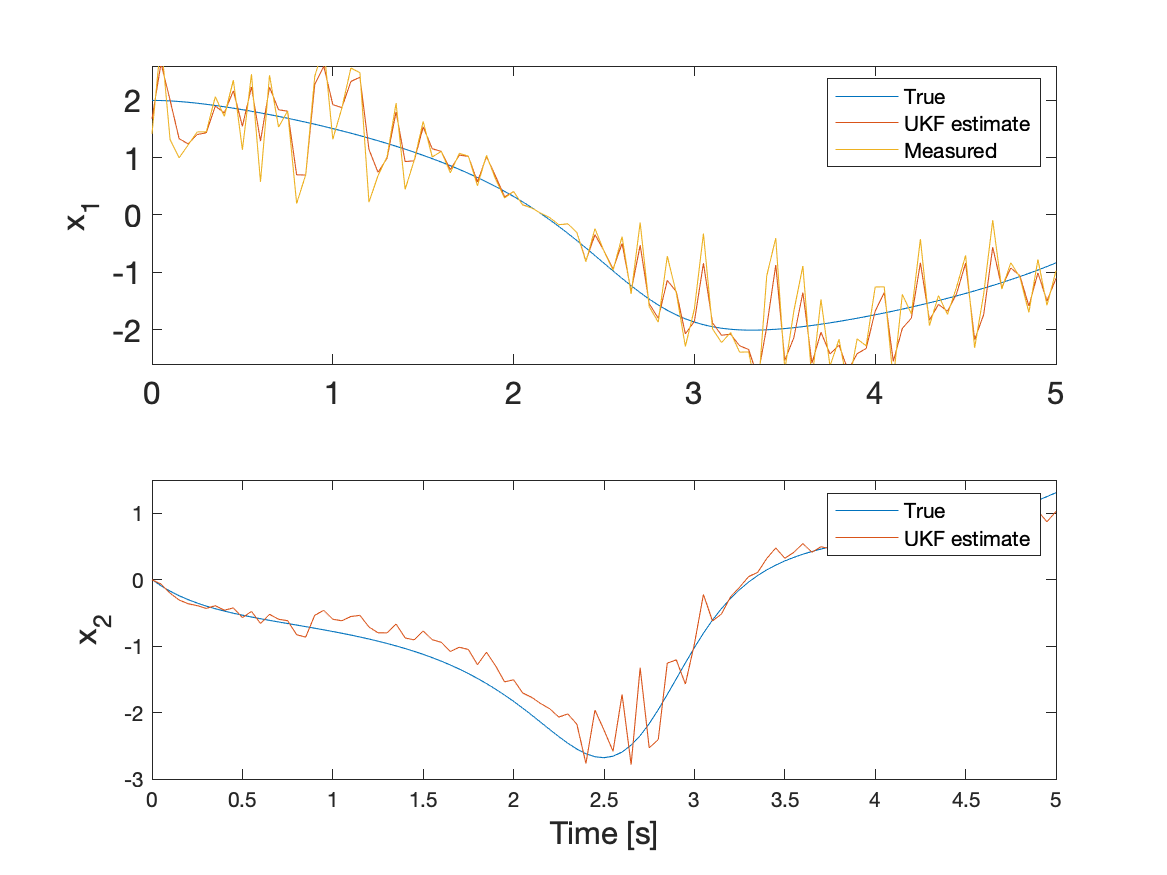
\includegraphics[width=0.5\textwidth]{VDP_highPN.png}\label{fig:f1}}
  \hfill
  \subfloat[UKF with low process noise (0.0001 0.0001)]{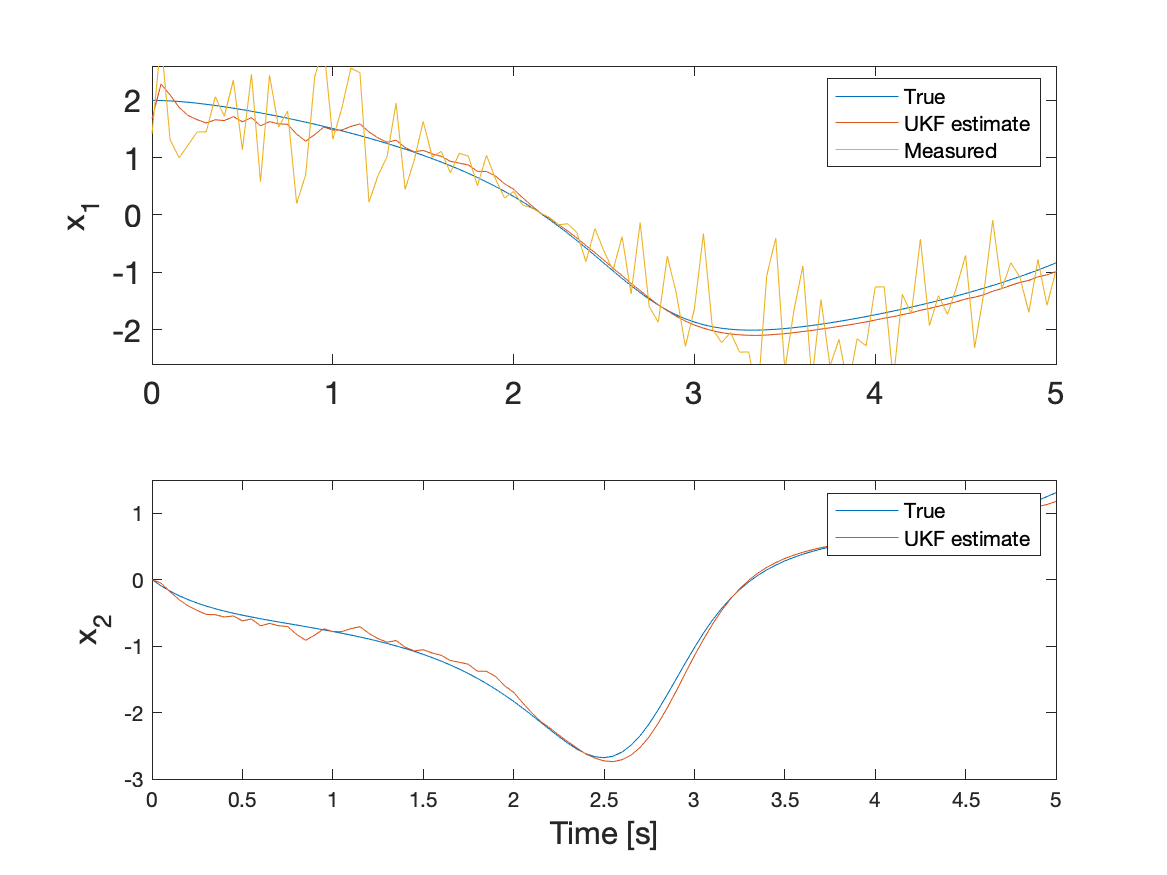
\includegraphics[width=0.5\textwidth]{VDP_lowPN.png}\label{fig:f2}}
  \caption{UKF on VDP oscillator with different values of process noise.
  Recall that process noise measures errors in the model. For the purpose of this example, process error was set to extreme high and low values. In theory, the Van der Pol equation should have small process error because it is a well used equation.}
   
\end{figure}
 
